\documentclass[12pt,a4paper,UTF8,fntef]{article}
\usepackage{ctex}
\usepackage{amsmath,amscd,amsbsy,amssymb,latexsym,url,bm,amsthm}
\usepackage[ruled,vlined]{algorithm2e}
\usepackage{graphicx,subfigure}
\usepackage{enumitem,balance,mathtools}
\usepackage{float}
\usepackage{wrapfig}
\usepackage{mathrsfs, euscript}
\usepackage[usenames]{xcolor}
\usepackage{hyperref}
\usepackage{epstopdf}
\usepackage{indentfirst}
\usepackage{breakcites}
\usepackage[numbers,sort&compress]{natbib}
\setlength{\oddsidemargin}{-0.365in}
\setlength{\evensidemargin}{-0.365in}
\setlength{\topmargin}{-0.5in}
\setlength{\headheight}{0.5in}
\setlength{\headsep}{0in}
\setlength{\textheight}{10.1in}
\setlength{\textwidth}{7in}
\newcommand{\upcite}[1]{\textsuperscript{\textsuperscript{\cite{#1}}}}
\hypersetup{
    colorlinks=true,
    linkcolor=black
}

\begin{document}
\begin{center}
\LARGE{\textbf{Machine Learning - Homework 1}}\vspace{1mm}\\
\footnotesize{Name: 史天尧 \qquad StudentID:517021910623}
\end{center}

\section{K-mean algorithm}
After initializing the center parameters $\mu_1$; $\mu_2$; $\cdots$; $\mu_K \in R_n$, the K-mean algorithm is to repeat the following two steps until convergence:
\begin{enumerate}
 \item Assign the points to the nearest $\mu_i$;
 \item Update $\mu_i$ to be the mean of the data points assigned to it.
\end{enumerate}
Prove that each of the above two steps will never increase the k-mean objective function,
\begin{equation}
J(\mu_K,\cdots,\mu_K)=\sum^N_{n=1}\sum^K_{k=1}r_{nk}\|x_n-\mu_k\|^2,
\end{equation}
where
\begin{equation}
	r_{nk}=\left\{\begin{matrix}
	1,&\quad \text{if }x_n\text{ is addigned to cluster } k;\\
	0,&\qquad \text{otherwise.}
	\end{matrix}\right.
\end{equation}

\textbf{Proof.}\quad We give the details of K-means algorithm to prove, that the objective function is non-increasing in every iteration and every stage.\newline
	\begin{algorithm}[H]
		\caption{K-means}
		\BlankLine
		Initialize $\mu_i,i=1,\cdots,K$\\
		\Repeat{$\mu_i$ converge for all $i$}{
		E-step:
		\For{all $x_n \in \chi$}{
		$r_{nk}\leftarrow\left\{\begin{matrix}
		1,&\quad \text{if }k=\arg\min_j\|x_n-\mu_j\|^2\\
		0,&\qquad \text{otherwise.}
		\end{matrix}\right.$
	}
	M-step:
	\For{all $\mu_k,k=1,\cdots,K$}{
$\mu_k \leftarrow \frac{\sum_n r_{nk}x_n}{\sum r_{nk}}$	
}
	}
	\end{algorithm}

Let $J(\mu_K,\cdots,\mu_K)^t$ be the value of the objective function immediately after $t$-th iteration and $J'(\mu_K,\cdots,\mu_K)^t$ be the value of that in $(t+1)$-th iteration after E-step but before M-step. (likewise for $r_{nk}$) We then show that 
$$
J(\mu_K,\cdots,\mu_K)^t\geq J'(\mu_K,\cdots,\mu_K)^t \geq J(\mu_K,\cdots,\mu_K)^{t+1}.
$$
After E-step, for all $x_n$, we have
$$
\sum_{k=1}^Kr'_{nk}|x_n-\mu_k\|^2=\min_j|x_n-\mu_j\|^2,
$$
which cannot be greater than $\sum_{k=1}^Kr_{nk}|x_n-\mu_k\|^2$ as the former result equals some $|x_n-\mu_j\|^2$. Therefore 
$$
J'(\mu_K,\cdots,\mu_K)^t=\sum_{n=1}^N\sum_{k=1}^Kr'_{nk}|x_n-\mu_k\|^2\leq \sum_{n=1}^N\sum_{k=1}^Kr_{nk}|x_n-\mu_k\|^2=J(\mu_K,\cdots,\mu_K)^t
$$
Then let us move to M-step. Compute the partial derivative of $\mu_k$ to $J$ and let it equal 0:
\begin{align*}
	\frac{\partial J}{\partial \mu_k}=&2\sum_{n=1}^Nr_{nk}(\mu_k-x_n)=0,\\
	\mu_k=&\frac{\sum_{n=1}^N r_{nk}x_n}{\sum_{n=1}^N r_{nk}}.
\end{align*}
Therefore in M-step, the value we assign to $\mu_k$ is exactly the extreme (minimal) point of $J$. And since $J$ is convex, it becomes the minimum point when $r_{nk}$s are fixed. From this point, we have $J'(\mu_K,\cdots,\mu_K)^t \geq J(\mu_K,\cdots,\mu_K)^{t+1}$. In conclusion, we have proved in each iteration and step, the objective function is non-increasing.\qed

\section{K-mean vs GMM}
Give a variant of k-mean algorithm somewhat between the original k-mean and Expectation-Maximization (EM) for Gaussian Mixture Models (GMM). Please specify the computational details of the formulas. Pseudo-codes of the algorithm would be great.

Discuss the advantages or limitations of your algorithm.

\textbf{Solution.} According to the lecture, this variant can be achieved via multiple approaches. ``GMM is more general then K-means by considering mixing weights, covariance matrices, and soft assignments.'' We can selectively save some feature(s) of GMM and derive a new algorithm. For example, we can modify GMM and let $\pi_i=1/k, \forall i$ in the initialization stage and fix it, namely preserving all features except mixing weights (prior estimate). 

Or we can let the covariance matrix be the identity matrix or multiplied by some constant, or a general diagonal matrix, assigning different weights to different dimensions of data. We can even abort the probabilistic frame but adopt Mahalanobis distance. Nevertheless, here we give an example of letting $\pi_i=1/k, \forall i$ and fix it.\newline
\begin{algorithm}[H]
	\caption{K-mean Variant}
	\BlankLine
	Initialize $\mathbf{\mu}_i, \mathbf{\Sigma}_i, i=1,\cdots,K$\\
	\Repeat{$\mu_i, \Sigma_i$ converge for all $i$}{
		E-step:
		\For{all $\mathbf{x}_n \in \chi$}{
			$\gamma(z_{nk})\leftarrow\frac{\mathcal{N}(\mathbf{x}_n|\mathbf{\mu}_k, \mathbf{\Sigma}_k)}{\sum\limits_{j=1}^K \mathcal{N}(\mathbf{x}_n|\mathbf{\mu}_j, \mathbf{\Sigma}_j)}$
		}
		M-step:
		\For{all $\mathbf{\mu}_k, \mathbf{\Sigma}_k,k=1,\cdots,K$}{
			$N_k \leftarrow \sum\limits_{n=1}^N \gamma(z_{nk})$\\
			$\mathbf{\mu}_k \leftarrow \frac{1}{N_k}\sum\limits_{n=1}^N \gamma(z_{nk})\mathbf{x}_n$	\\
			$\mathbf{\Sigma}_k \leftarrow \frac{1}{N_k}\sum\limits_{n=1}^N \gamma(z_{nk})(\mathbf{x}_n-\mathbf{\mu}_k)(\mathbf{x}_n-\mathbf{\mu}_k)^{\text{T}}$
		}
	}
\end{algorithm}

Advantage of the algorithm includes soft assigning and capturing anisotropy among different dimensions of data. Soft assigning can, to some extent, relive the hungry / dead centroid problem caused by bad initialization, and better describes data points which are in the middle of several clusters: that they do not belong to a certain cluster, but several in between. Capturing anisotropy makes the algorithm better adapted to real-life data, as different dimensions of them usually have different semantics, some of which can be very different in scales.

Disadvantage of this algorithm is also clear: it aborts $\pi_k$, thus denying prior knowledge of possible clusters. In practice, domain-specific and expert knowledge is often leveraged as prior to make the performance better. 
\section{K-mean vs CL}
Compare the k-mean algorithm with competitive learning (CL) algorithm. Could you apply the idea of Rival Penalized Competitive Learning (RPCL) to k-mean so that the number of clusters is automatically determined? If so, give the details of your algorithm and then implement it on a three-cluster dataset generated by yourself. If not, state the reasons.

\textbf{Solution.} We have already seen that RPCL can automatically delete redundant clusters when the manually selected $k$ is larger than the actual number of clusters. Each cluster only pulls one $\mu_i$, i.e. the winner near its center, but pushes rivals away, thus determining the number of clusters automatically. However, when the manually selected $k$ is smaller than the actual number of clusters, RPCL does not give an solution to add more clusters. A simple idea would be that to divide the large clusters (i.e. in fact two or more actual clusters, appearing to have large variation) into several smaller clusters, which can be implemented by conducting a $k=2$ K-means on large clusters, until no cluster is such large.

Therefore, we can conduct RPCL on the dataset at first, delete redundant clusters or split excessively large clusters after converged, and use the result as initialization of the final K-means pass. Here we give the algorithm:
\newline
\begin{algorithm}[H]
	\caption{RPCL based K-mean}
	\BlankLine
	Initialize $\mathbf{\mu}_i, i=1,\cdots,K$, max iteration $T$, threshold of number of data points belong to a cluster $N_{\min}$ (below which is redundant and to be deleted), threshold of variation of a cluster $\sigma_{\max}$ (above which to be split);\\
	\Repeat{iteration $<T$ and $\mu_i$ converge for all $i$}{
			Conduct RPCL ;
	}
	Assign all data points to their nearest $\mu_i$ (E-step);\\
	\While{no cluster's variation $\geq \sigma_{\max}$}{
	\For{all clusters}{
		\If{number of data points assigned  $<N_{\min}$}{delete this cluster;}
		\If{variation $\geq \sigma_{\max}$}{conduct $k=2$ K-mean on this cluster, replace the original center with results derived from K-mean;}
	}
	}
Use the results $\mathbf{\mu}_i, i=1,\cdots,K'$ as initialization of normal K-mean, conduct K-mean.
\end{algorithm}

The experiment (and in Problem 4) is carried out using Python and scikit-learn package. To better visualize the result, we generate a 90 samples, 2-dimensional and 3-cluster dataset from Gaussian distributions. Set $k=5$, and the result is:
\begin{figure}[!h]
	\centering
	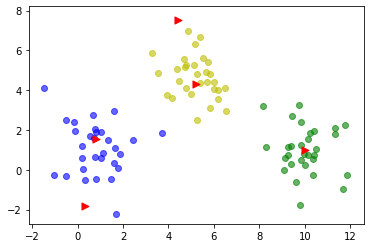
\includegraphics[width=0.7\textwidth]{untitled.png}
\end{figure}
\section{Model Selection of GMM}
Write a report on experimental comparisons on model selection performance between BIC,AIC and VBEM.

Specifically, you need to randomly generate datasets based on GMM, by varying some factors, e.g., sample sizes, dimensionality, number of clusters, and so on.
\begin{enumerate}
	\item BIC, AIC: First, run EM algorithm on each dataset $X$ for $k=1,\cdots,K$ and calculate the log-likelihood value $\ln[p(X|\hat{\Theta}_k)]$ is the maximum likelihood estimate for parameters; Second, select the optimal $k^*$ by
	\begin{equation}
		k^*={\arg\max}_{k=1,\cdots,K}J(k),
	\end{equation}
	\begin{equation}
		J_{AIC}(k)=\ln[p(X|\hat{\Theta}_k)]-d_m,
	\end{equation}
	\begin{equation}
	J_{BIC}(k)=\ln[p(X|\hat{\Theta}_k)]-\frac{\ln N}{2}d_m.
	\end{equation}
	\item Use VBEM algorithm for GMM to select the optimal $k^*$ automatically or via evaluating the lower bound.
\end{enumerate}

\textbf{Solution.} We carry out the comparisons following the sequence of different datasets:
\begin{enumerate}
	\item \textbf{Dimensionality=2, Sample size=500 for each cluster, Number of clusters=2}
	\begin{itemize}
		\item \textbf{AIC}
		\begin{figure}[!h]
			\centering
			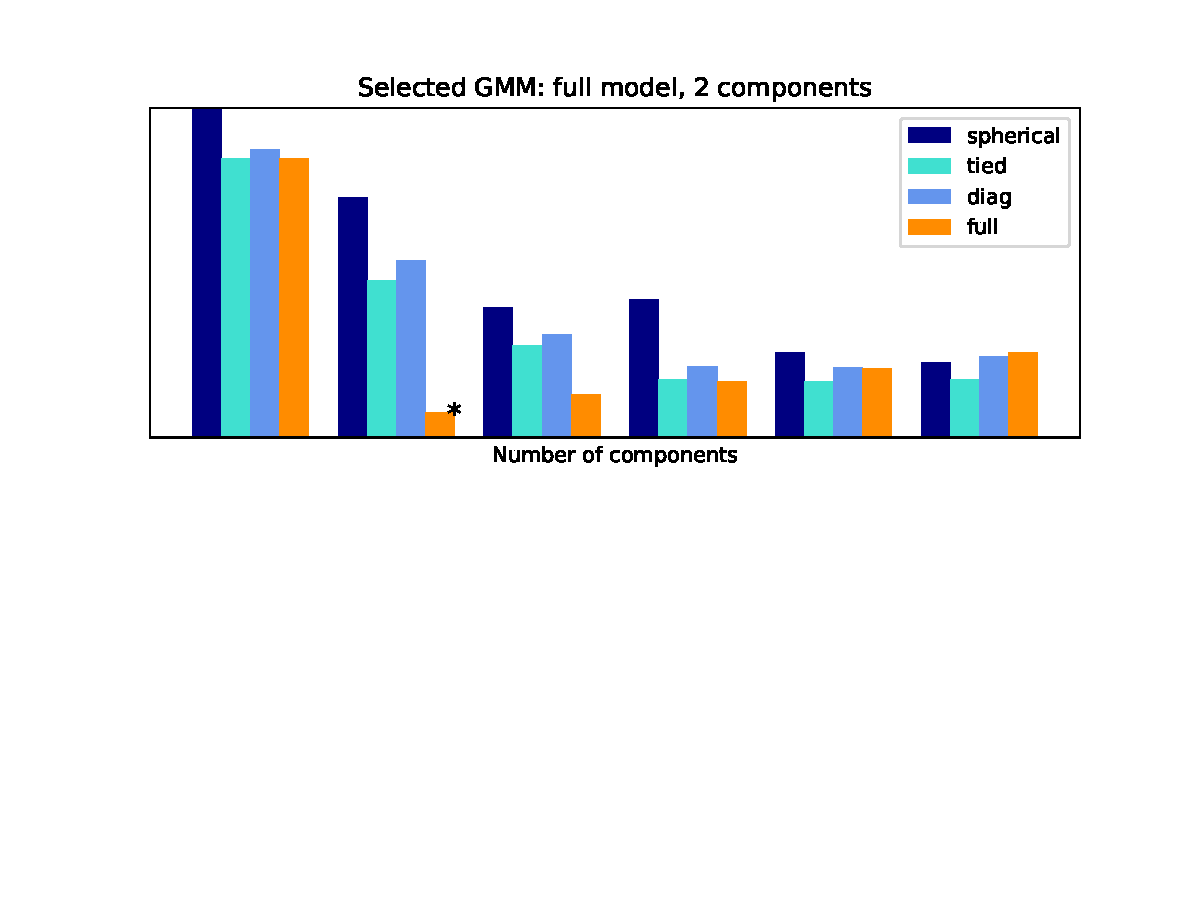
\includegraphics[width=0.7\textwidth]{AIC_1.pdf}
			\caption{AIC for choosing $k^*$ in dataset 1}
		\end{figure}
		\item \textbf{BIC}
		\begin{figure}[!h]
			\centering
			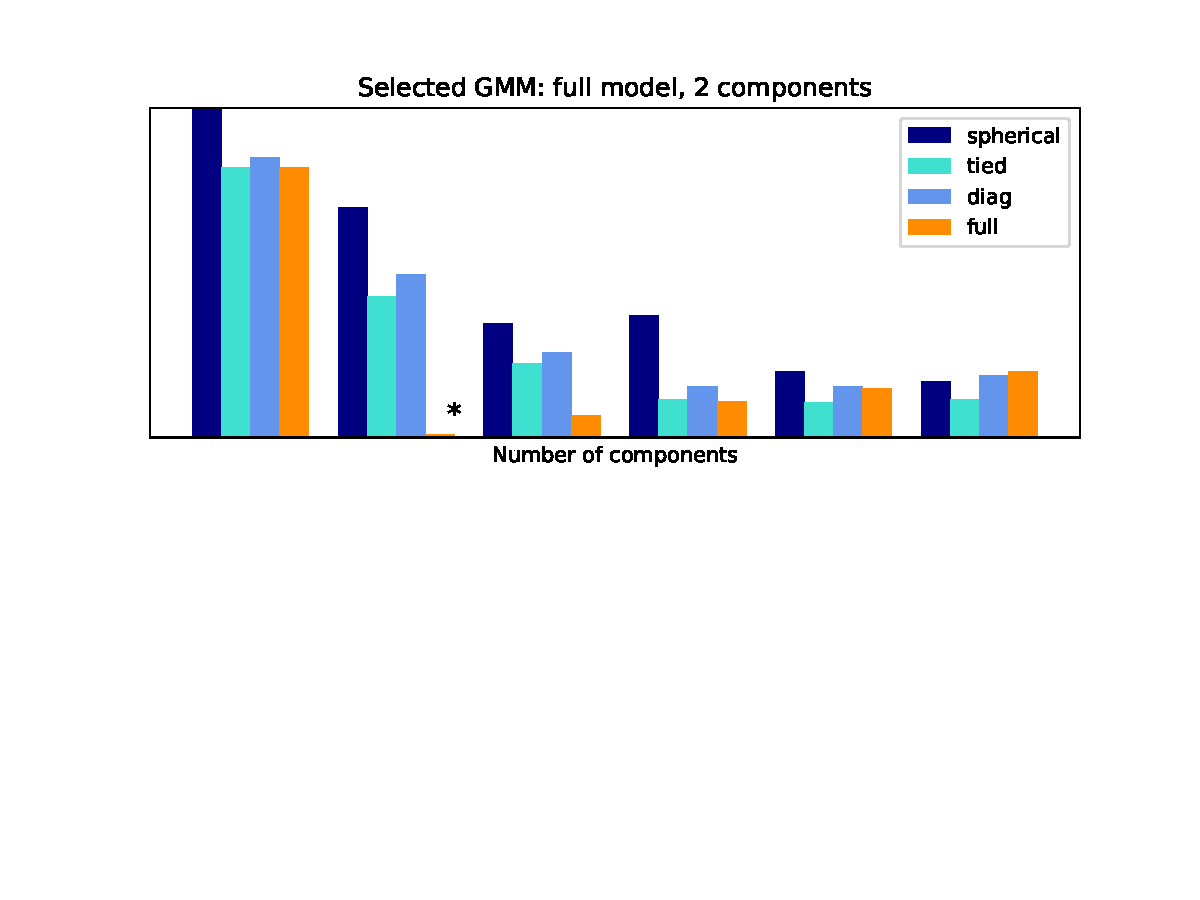
\includegraphics[width=0.7\textwidth]{BIC_1.pdf}
			\caption{BIC for choosing $k^*$ in dataset 1}
		\end{figure}
	
	AIC and BIC creterion give the same GMM model in this dataset. Below is the visualization. However, we can see that BIC is less likely to choose wrong $k^*$.
	\newpage
	\begin{figure}[!h]
		\centering
		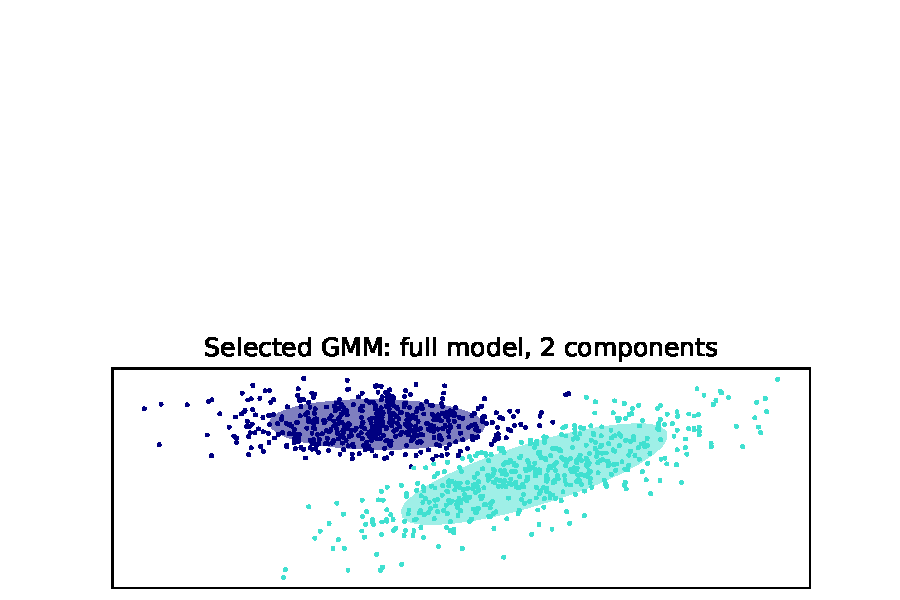
\includegraphics[width=0.7\textwidth]{GMM_1.pdf}
		\caption{The chosen GMM in dataset 1}
	\end{figure}
	\item \textbf{VBEM}\newline
	As implied in the VBEM algorithm, take a conservative stand, and fit only the most possible components. However, when testing on this dataset, it goes into problems. As shown below, it only partly works when selecting $k=5$, and VBEM can tell there is one redundant cluster. But for $k=3,4$, it is not satisfying.
	\begin{figure}[!h]
		\centering
		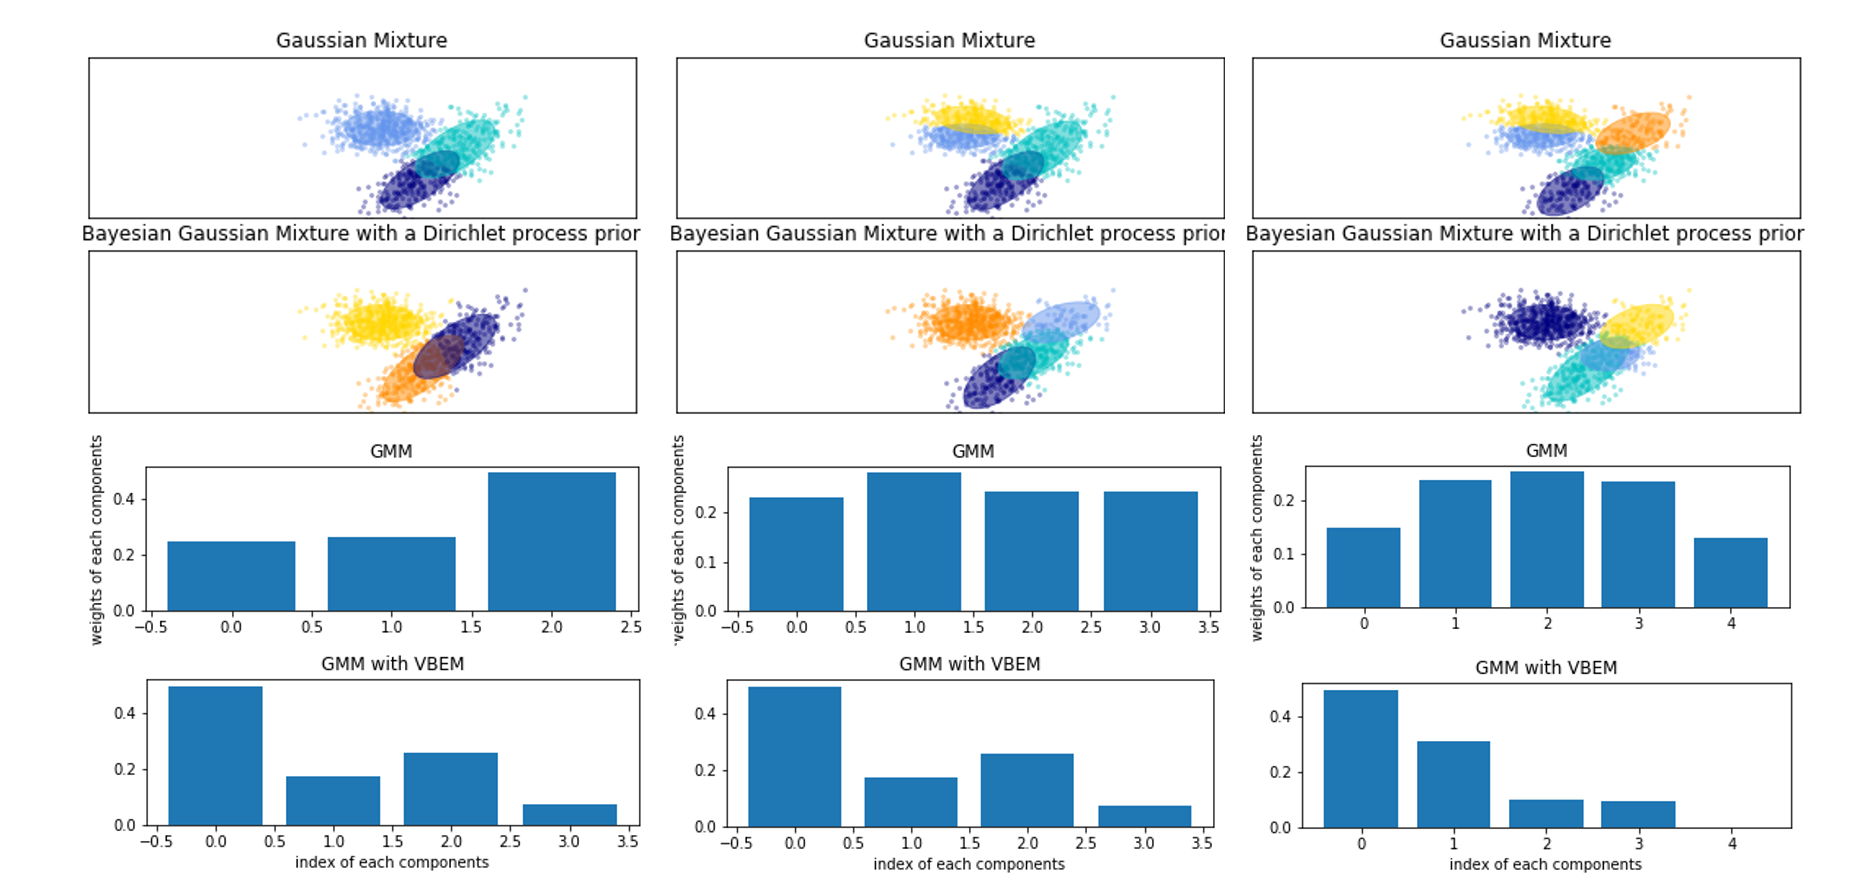
\includegraphics[width=0.9\textwidth]{VBEM_1.png}
		\caption{VBEM for $k=3,4,5$ in dataset 1}
	\end{figure}
	
	Why does this happen? I try to modify the dataset and pull the two cluster away. This time, the VBEM works. This implies that when the clusters are actually close to each other, VBEM may fail to tell out the redundant clusters. Or in other words, there is not enough evidence for VBEM to reduce clusters, as the number provided seems just fine.
	\begin{figure}[!h]
		\centering
		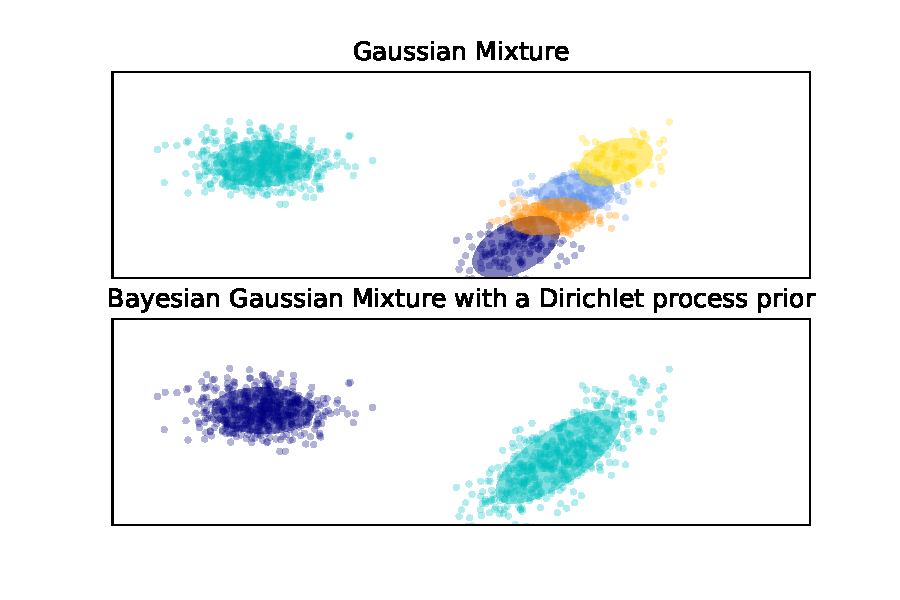
\includegraphics[width=0.7\textwidth]{VBEM_1_4.pdf}
		\caption{VBEM vs GMM in modified dataset 1}
	\end{figure}
	\end{itemize}
	\item \textbf{Dimensionality=2, Sample size=1000 for each cluster, Number of clusters=2}
	\begin{itemize}
		\item \textbf{AIC}
		\begin{figure}[!h]
			\centering
			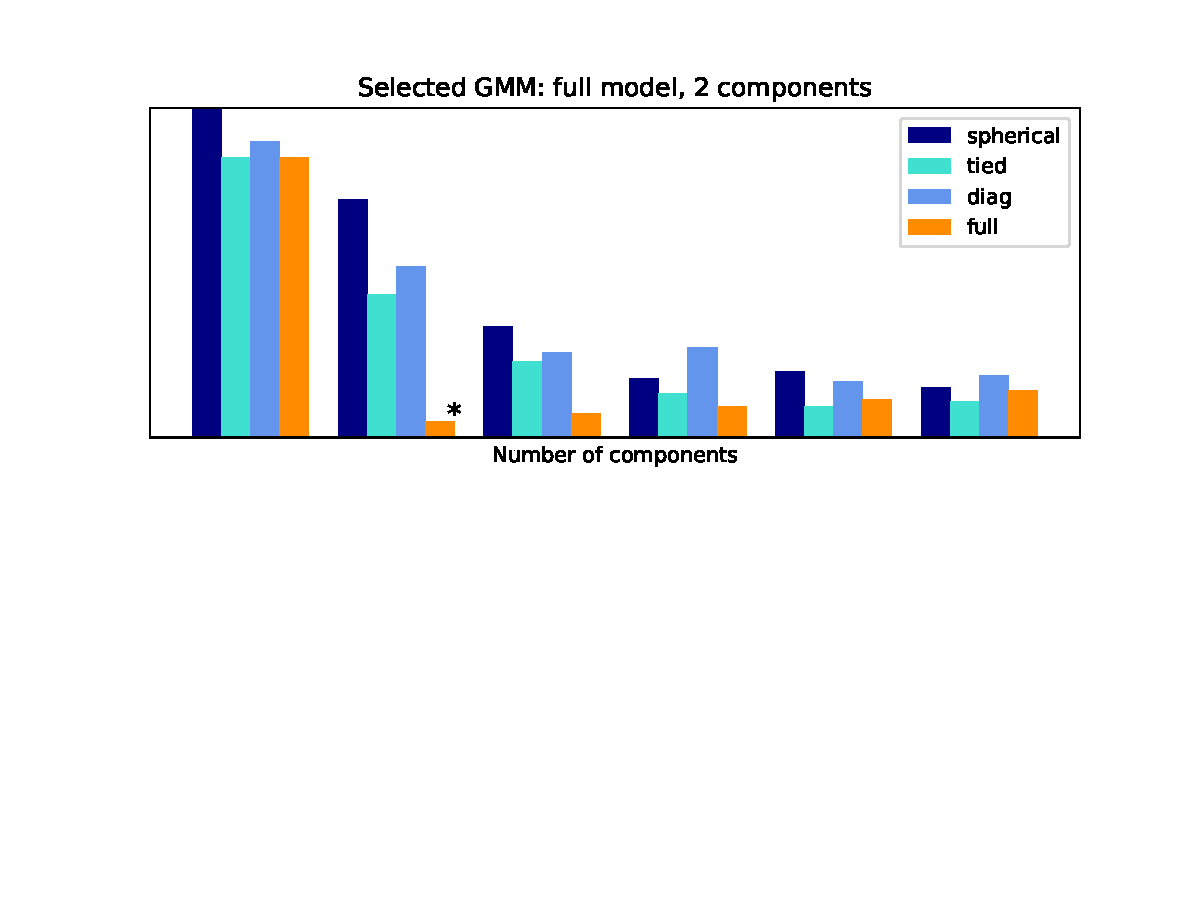
\includegraphics[width=0.7\textwidth]{AIC_2.pdf}
			\caption{AIC for choosing $k^*$ in dataset 2}
		\end{figure}
		\item \textbf{BIC}
		\begin{figure}[!h]
			\centering
			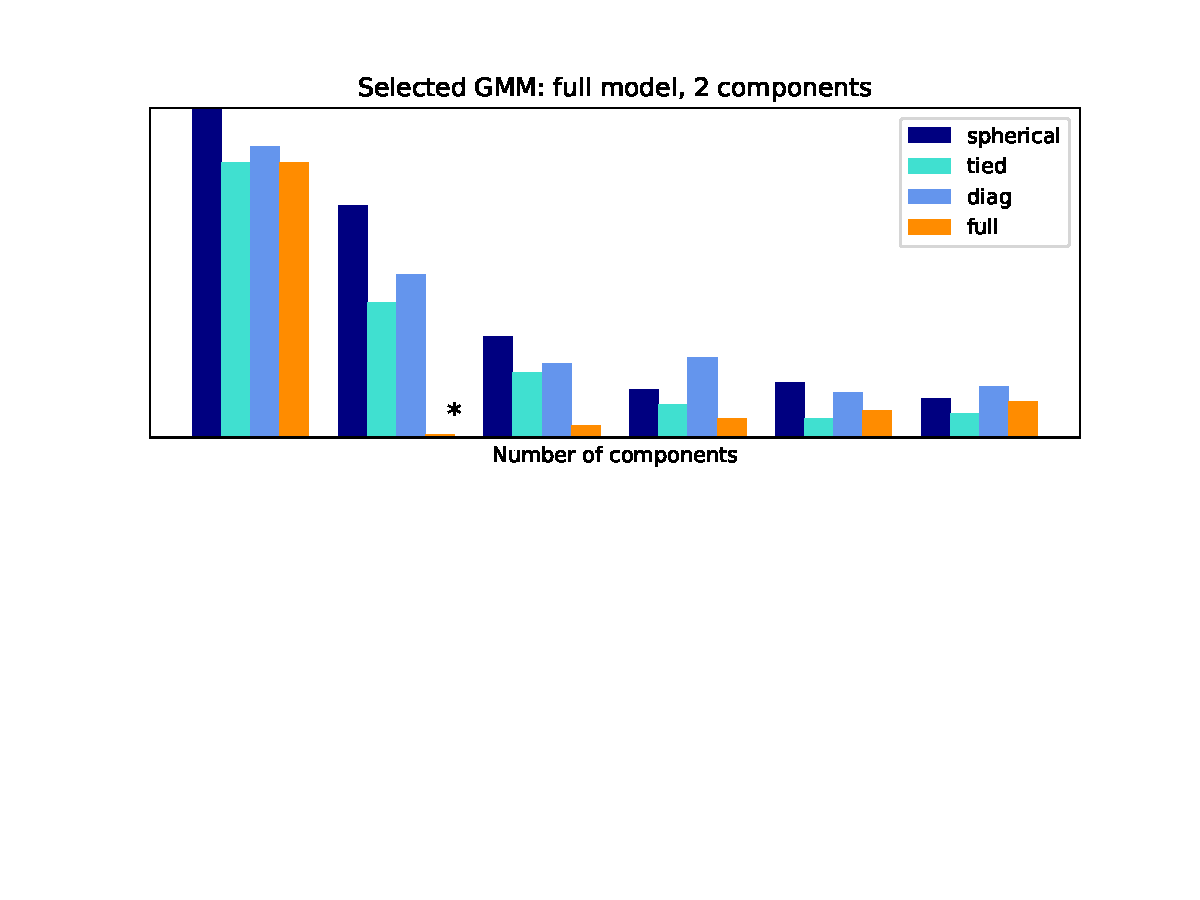
\includegraphics[width=0.7\textwidth]{BIC_2.pdf}
			\caption{BIC for choosing $k^*$ in dataset 2}
		\end{figure}
		
		The pattern is the same as in dataset 1.\newpage
		\begin{figure}[!h]
			\centering
			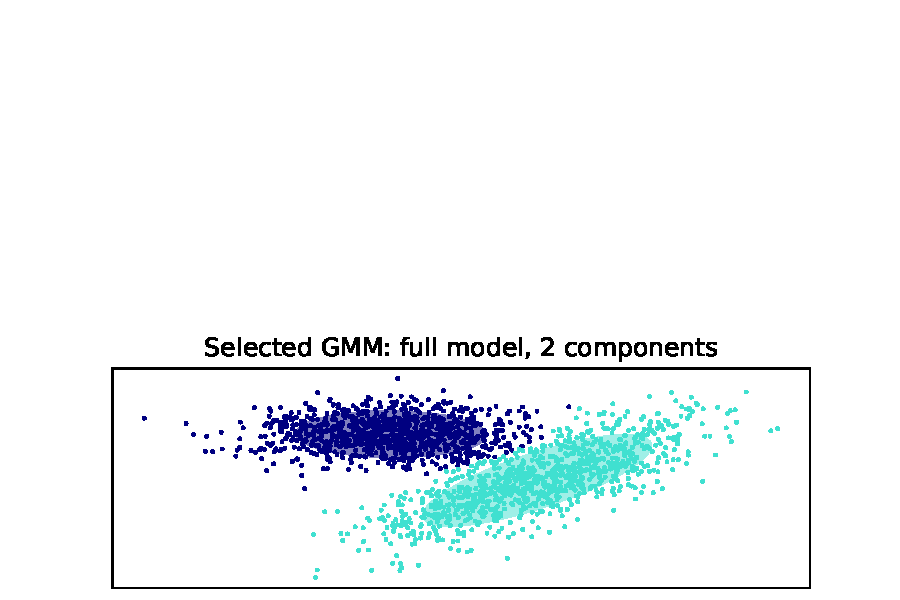
\includegraphics[width=0.7\textwidth]{GMM_2.pdf}
			\caption{The chosen GMM in dataset 2}
		\end{figure}
		\item \textbf{VBEM}\newline
		The same problem happens, or even worsens this time\textemdash as the sample size increases, there are more outliers and harder for VBEM to tell. Even though the two clusters are pulled away, VBEM still fits one redundant cluster.
		\begin{figure}[!h]
			\centering
			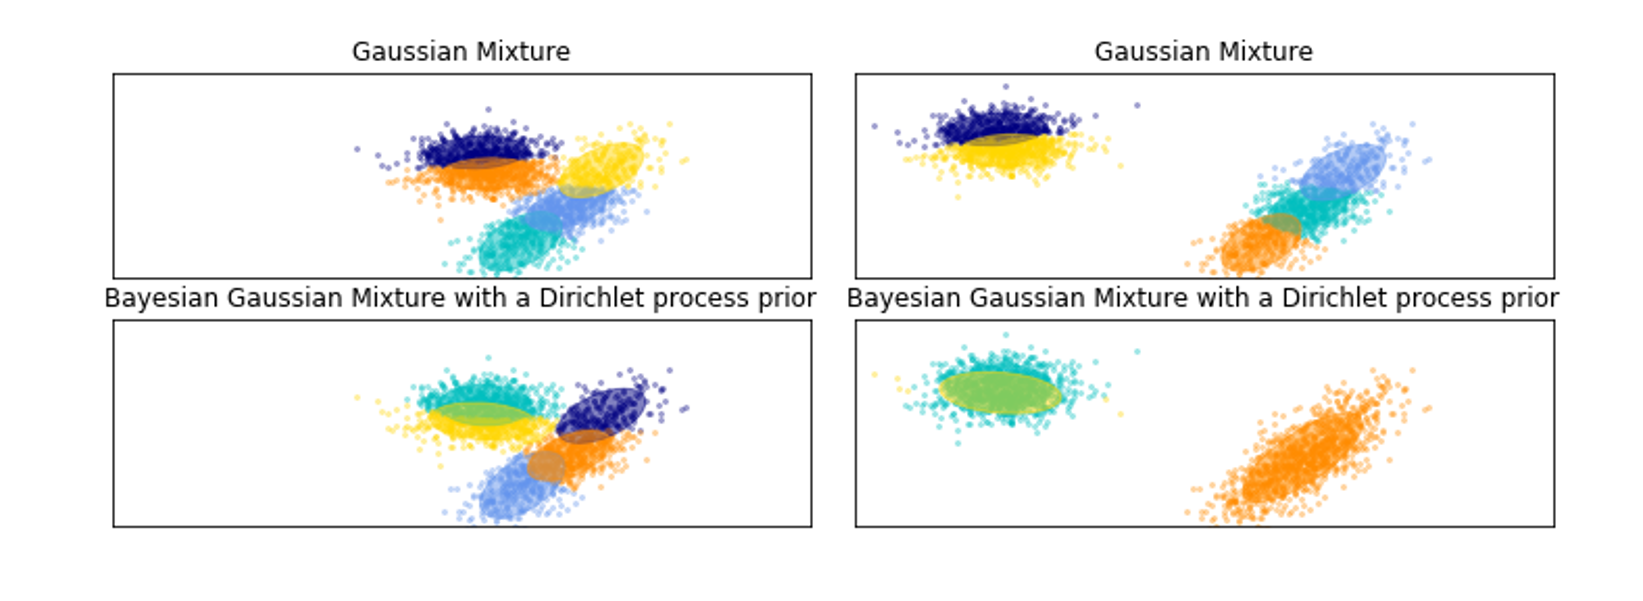
\includegraphics[width=\textwidth]{VBEM_2.png}
			\caption{VBEM vs GMM in original and modified Dataset 2}
		\end{figure}
	\end{itemize}
\item \textbf{Dimensionality=2, Sample size=1000 for each cluster, Number of clusters=3}
\begin{itemize}
	\item \textbf{AIC}
	\begin{figure}[!h]
		\centering
		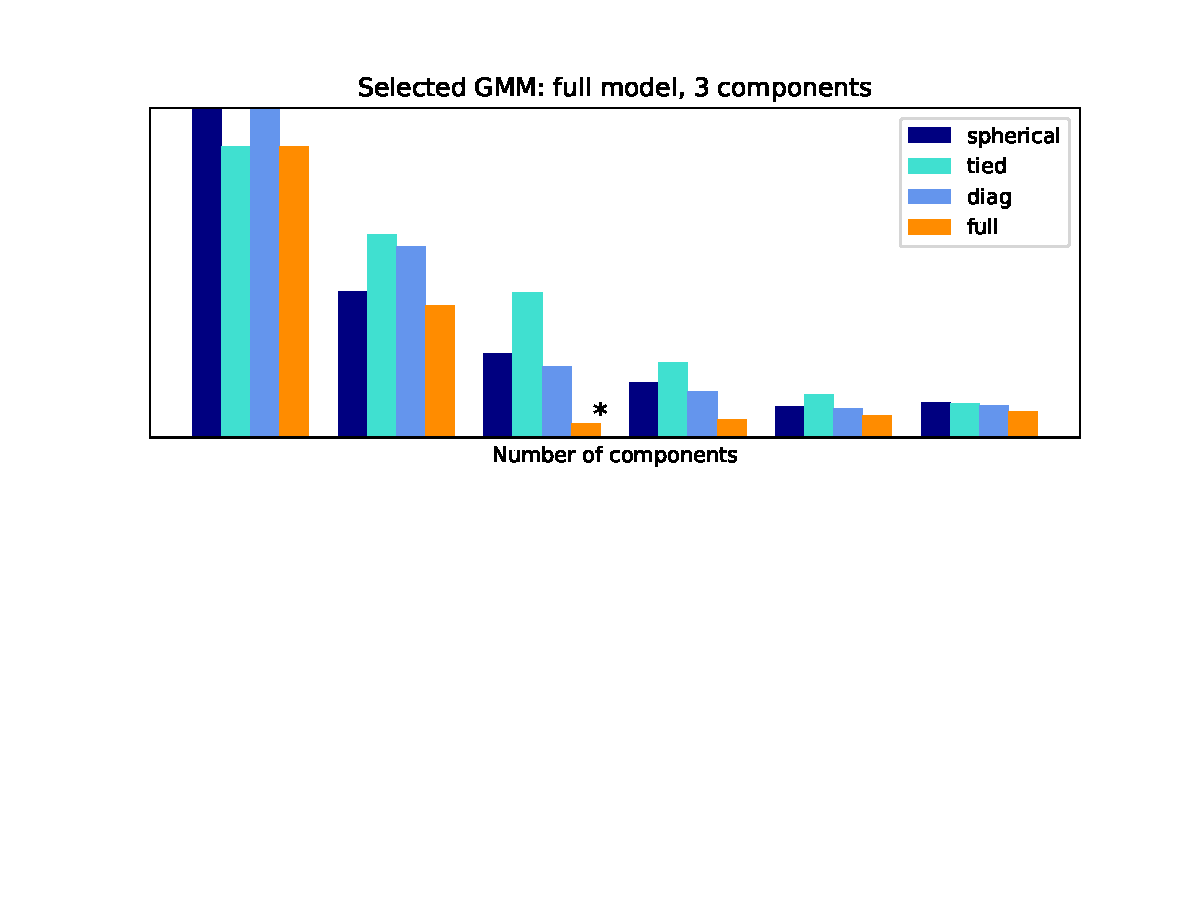
\includegraphics[width=0.7\textwidth]{AIC_3.pdf}
		\caption{AIC for choosing $k^*$ in dataset 3}
	\end{figure}
	\item \textbf{BIC}
	\begin{figure}[!h]
		\centering
		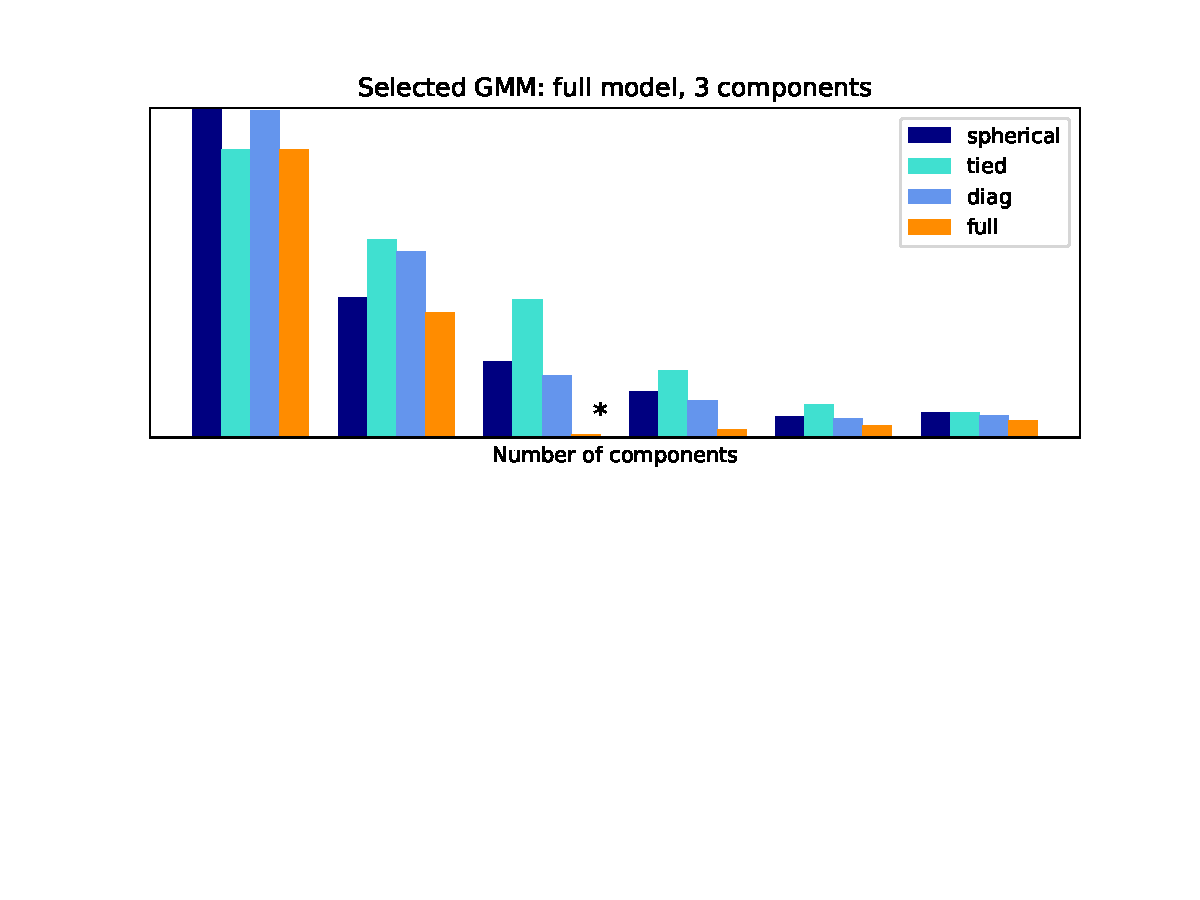
\includegraphics[width=0.7\textwidth]{BIC_3.pdf}
		\caption{BIC for choosing $k^*$ in dataset 3}
	\end{figure}
	
	The pattern is the same as in dataset 1.
	\begin{figure}[!h]
		\centering
		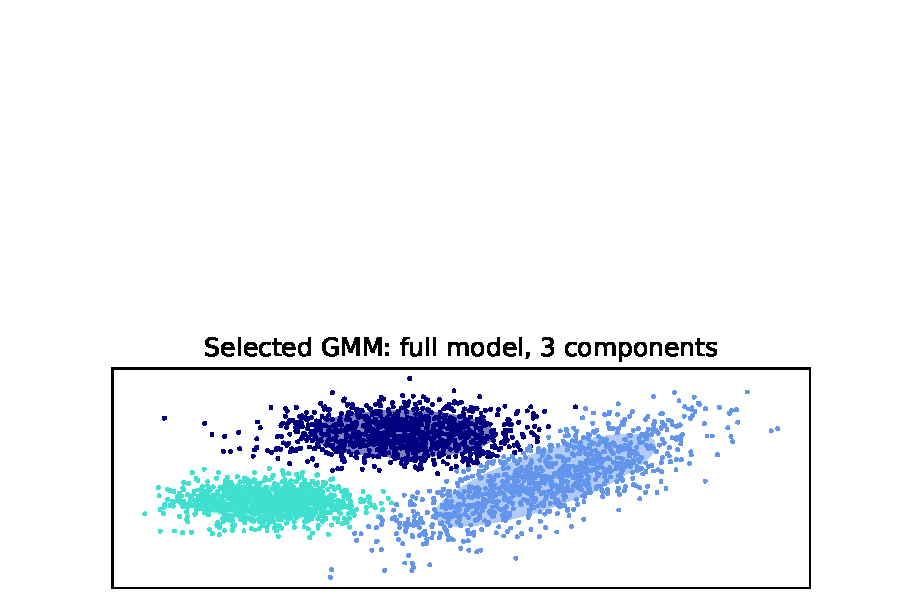
\includegraphics[width=0.7\textwidth]{GMM_3.pdf}
		\caption{The chosen GMM in dataset 3}
	\end{figure}
	\item \textbf{VBEM}\newline
	The pattern is the same as in dataset 1. Better than in dataset 2, maybe because of the decreased $k/\#cluster$ ratio. This implies that determining $k$ automatically is really tricky and relies on setting of some key parameters.\newpage
	\begin{figure}[!h]
		\centering
		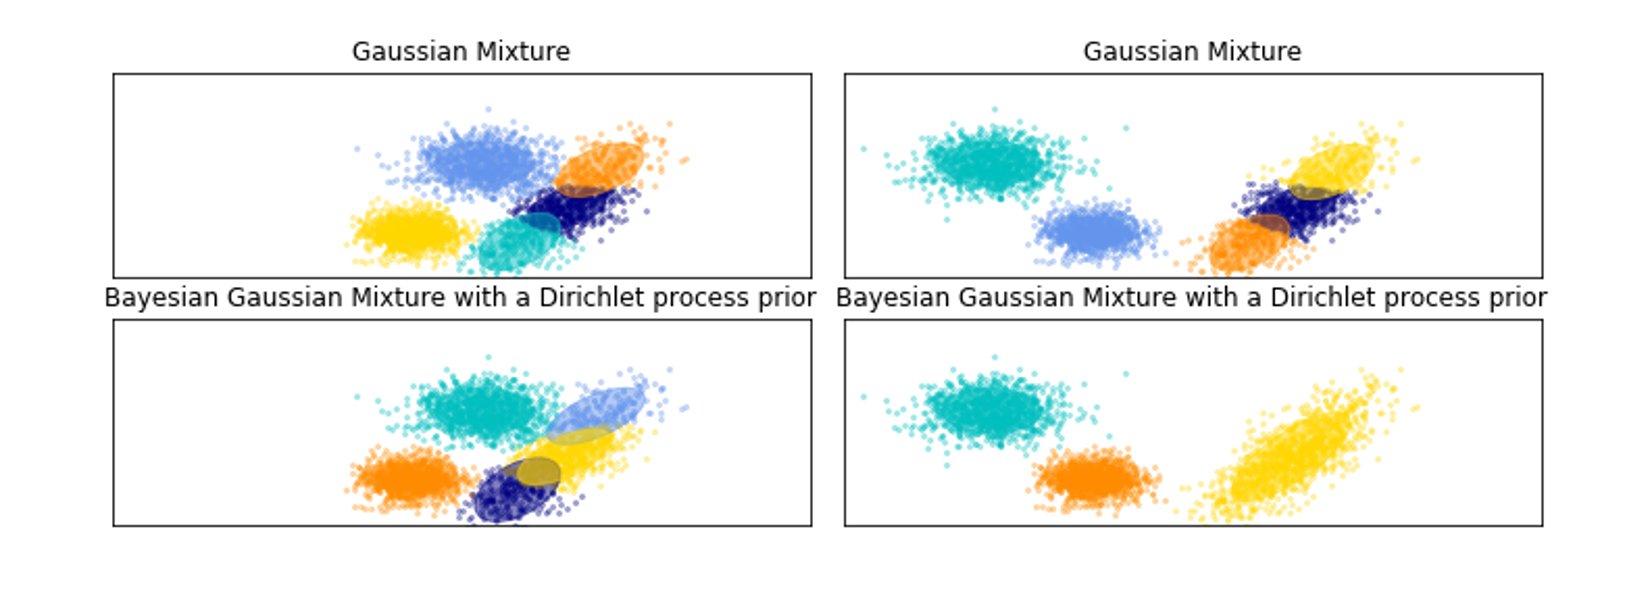
\includegraphics[width=\textwidth]{VBEM_3.png}
		\caption{VBEM vs GMM in original and modified Dataset 3}
	\end{figure}
	\begin{figure}[!h]
		\centering
		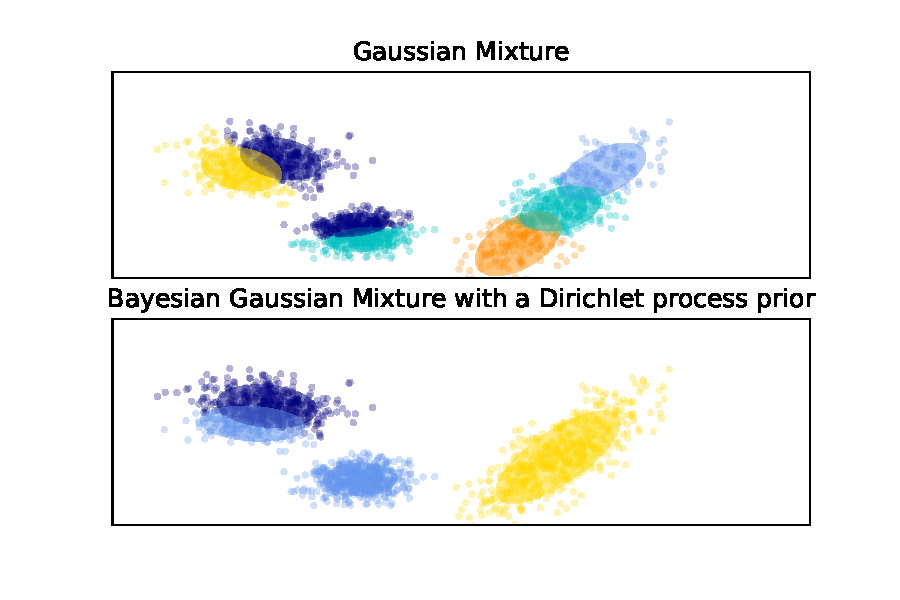
\includegraphics[width=0.7\textwidth]{VBEM_3_3.pdf}
		\caption{VBEM fails again when $k$ set to 7}
	\end{figure}
\end{itemize}
\item \textbf{Dimensionality=10, Sample size=500 for each cluster, Number of clusters=2}
\begin{itemize}
	\item \textbf{AIC}
	\begin{figure}[!h]
		\centering
		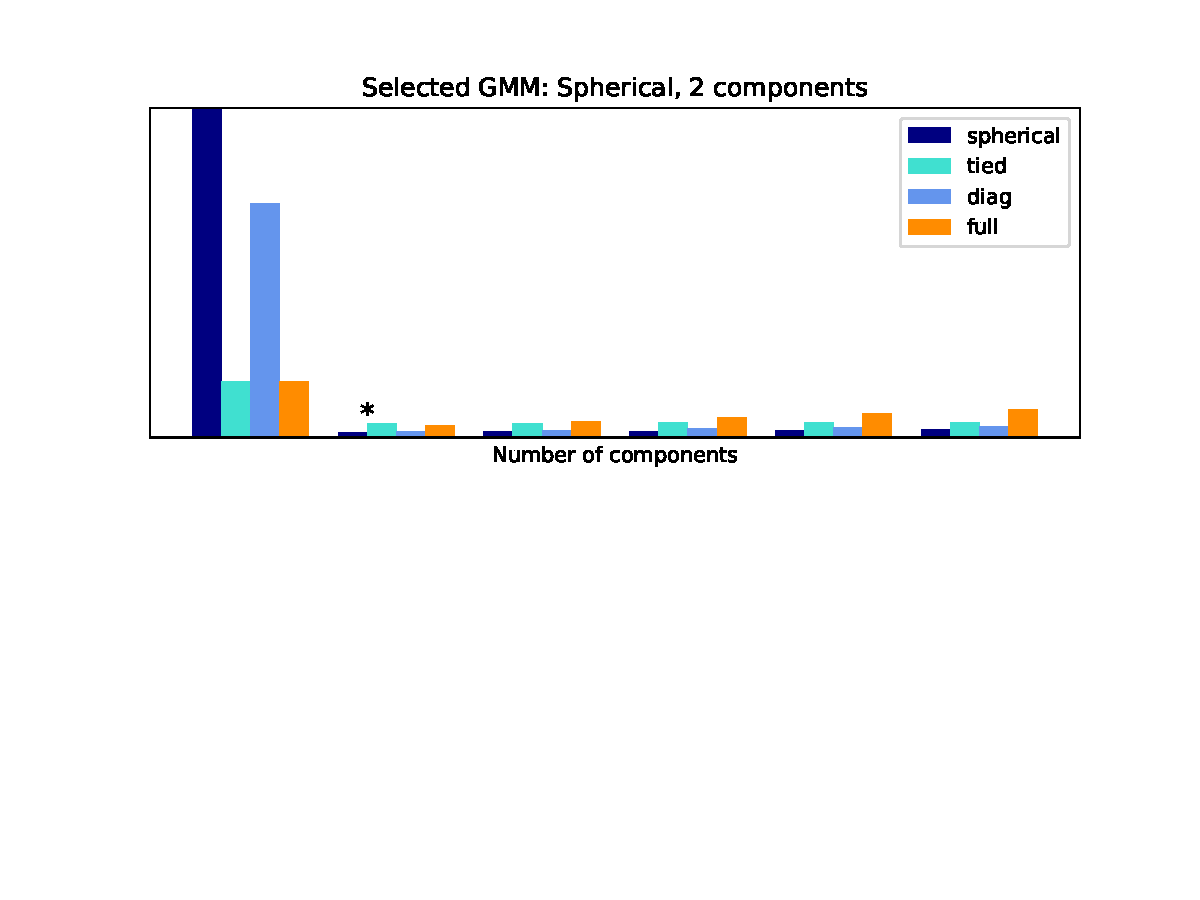
\includegraphics[width=0.7\textwidth]{AIC_4.pdf}
		\caption{AIC for choosing $k^*$ in dataset 4}
	\end{figure}
	\item \textbf{BIC}
	\begin{figure}[!h]
		\centering
		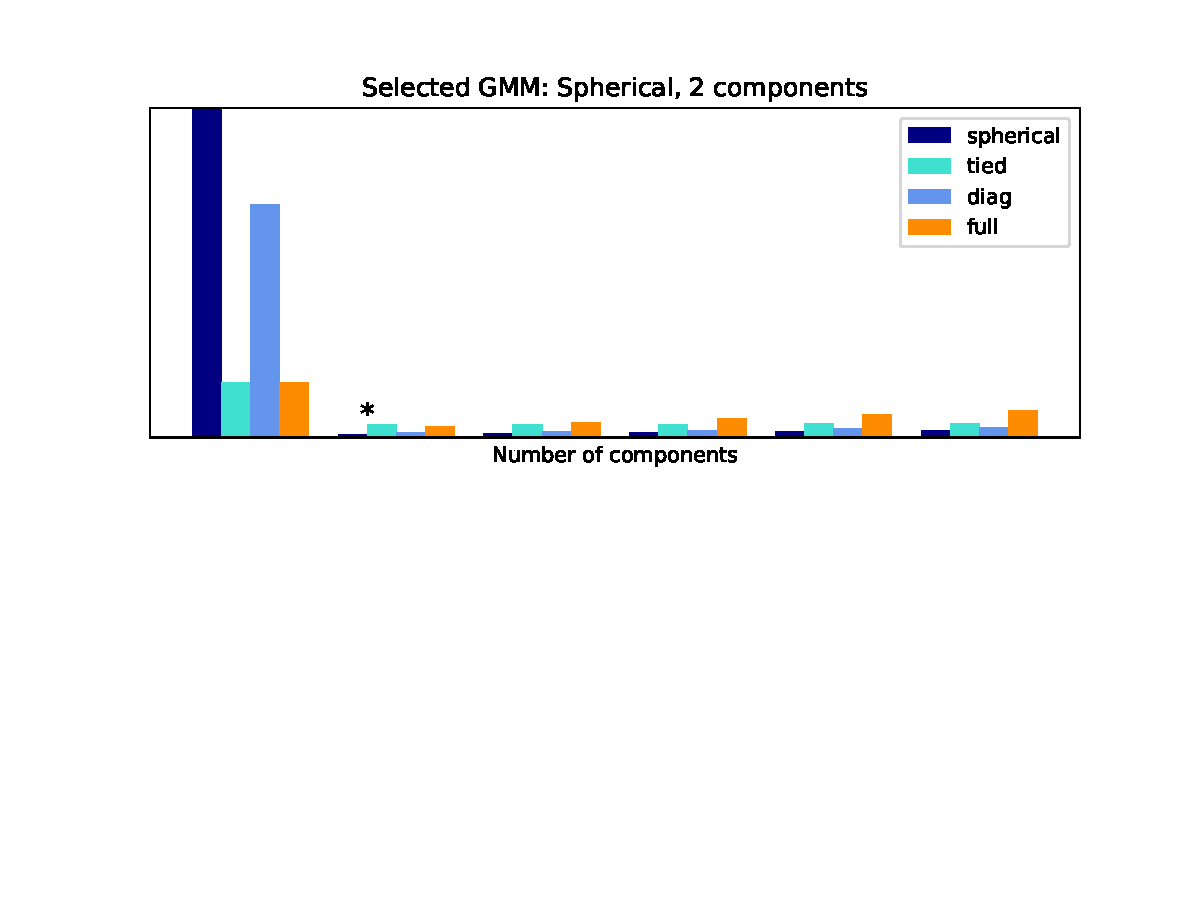
\includegraphics[width=0.7\textwidth]{BIC_4.pdf}
		\caption{BIC for choosing $k^*$ in dataset 4}
	\end{figure}
	
	10-dimensional data cannot be visualized, though AIC and BIC still agree with each other. A major change is that spherical model is selected, which agrees with the way I generated 10-dim data\textemdash for convenience I did not apply transformation to the data drawn from the standard Gaussian distribution.
	\item \textbf{VBEM}\newline
	This time VBEM performs fairly\textemdash better than low dimensional results, though unable to reduce all redundant clusters, but keeps all redundant clusters very small (weight of cluster 2 is not 0).
	\begin{figure}[!h]
		\centering
		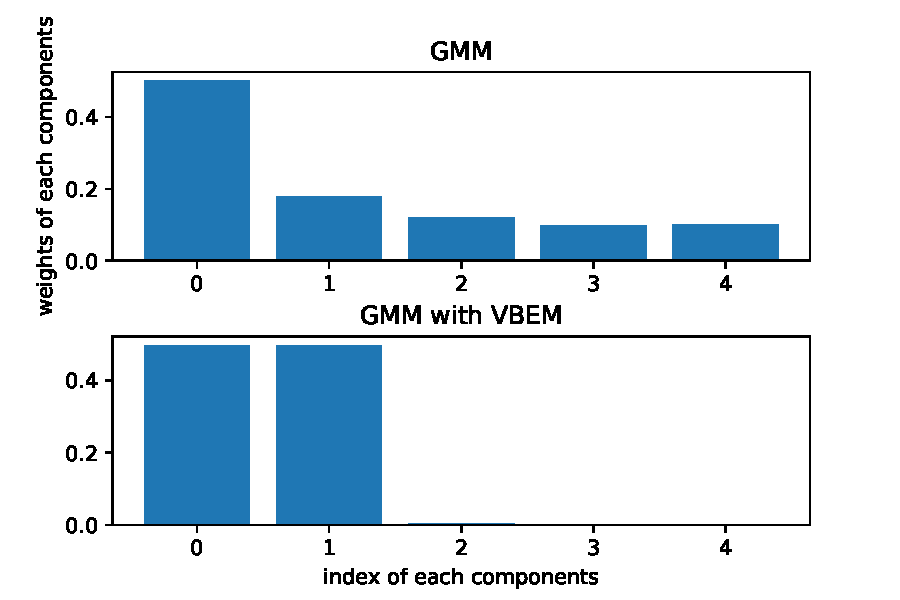
\includegraphics[width=0.7\textwidth]{VBEM_4.pdf}
		\caption{VBEM for choosing $k^*$ in dataset 4}
	\end{figure}
\end{itemize}
\end{enumerate}
\end{document}
